\section{Elektrochemie - Marco}

\subsection{Galvanische Zelle}
Grundprinzip: Oxidation und Reduktion sind räumlich getrennt. \\
Anode: Ort der Oxidation \\
Kathode: Ort der Reduktion \\

Daniell-Element:
\begin{figure}[htbp!]
	\centering
	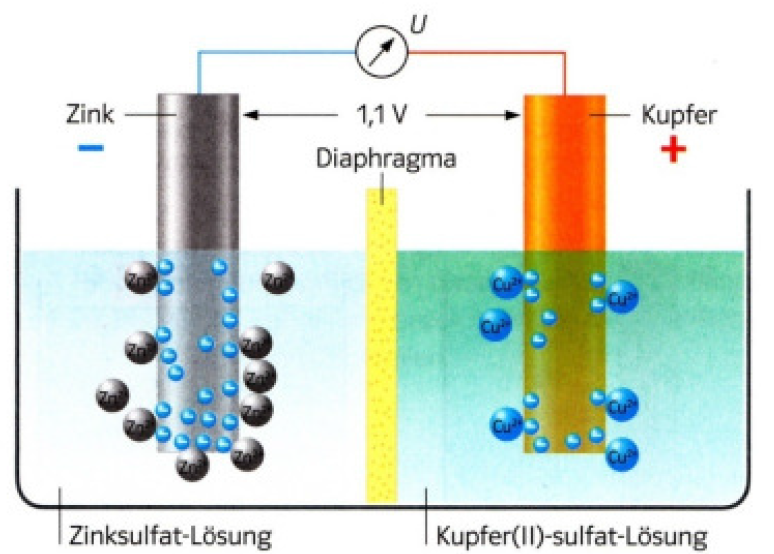
\includegraphics[width=0.7\linewidth]{images/10_Daniell_Element.png}
\end{figure}

Spannung $\Delta E = E_\text{Kathode}-E_\text{Anode}$ \\

Reaktionen:\\
Zink-Halbzelle (Anode): $Zn \leftrightarrow Zn^{2+} + 2 e^-$ \\
Kupfer-Halbzelle (Kathode): $Cu^{2+} + 2 e^- \leftrightarrow Cu$ \\

\subsubsection{Standard-Wasserstoffelektrode}
Referenzmessung des Redoxpotentials

\begin{figure}[htbp!]
	\centering
	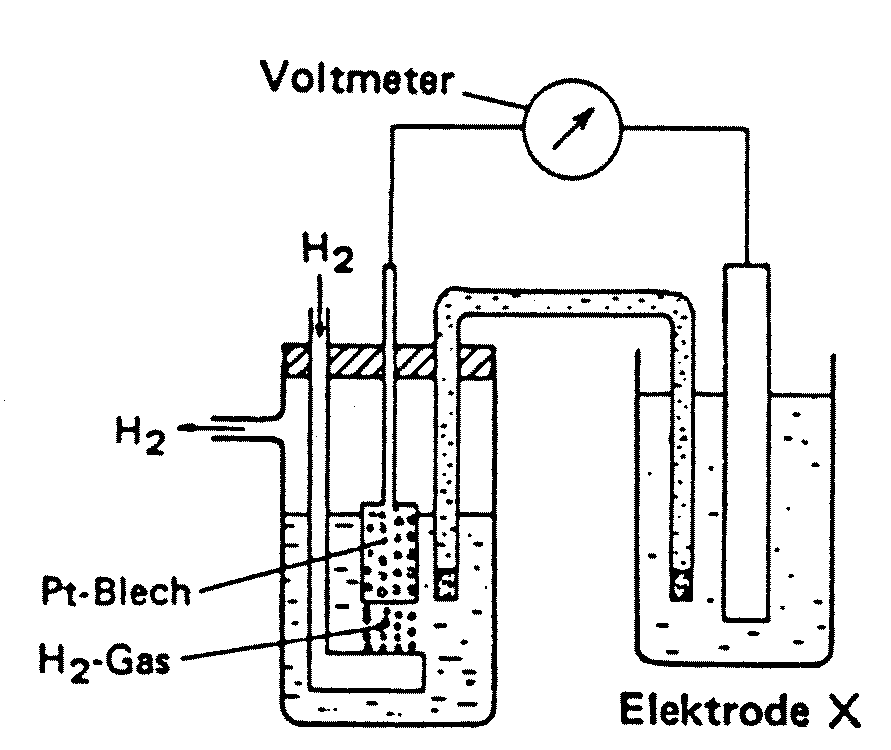
\includegraphics[width=0.6\linewidth]{images/10_Wasserstoffelektrode.png}
\end{figure}

Standardbedingungen:\\
p($H_2$) = 1013mbar, T=25$^\circ C$, Konzentration $[H_3O^+]$ = 1mol/l, $E^0(H_2/H_3O^+) = 0.0V$

Reaktionen: \\
Wasserstoff-Halbzelle: $H_2 + 2H_2O \leftrightarrow 2 H_3O^+ + 2 e^-$ \\
Halbzelle: $Me^{z+} + z e^- \leftrightarrow Me_{(s)}$ \\


\subsection{Edle und unedle Metalle}
\emph{Edle} Metalle: $E^0 > 0V$, zeigen kaum Reaktion mit $O_2, H_2O$, Säuren. Kommen gediegen in der Natur vor. \\

\emph{Unedle} Metalle: $E^0 < 0V$, gehen mit vielen Stoffen Reaktionen ein. Kommen in der Natur nur in Form von Verbindungen vor. \\

\subsection{Konzentrationsabhängigkeit des Redoxpotentials}
Das Redoxpotential ist u.a. von Temperatur, Druck, pH-Wert und Ionenkonzentration der Lösung vor. Das effektive Redoxpotential wird gemäss der \emph{Nernst}-Gleichung beschrieben:
\begin{eqnarray*}
	E_{RM/OM} &= E^0_{RM/OM} + \frac{R \cdot T}{z \cdot F} \cdot \ln\frac{[OM]}{[RM]} \\ &=  E^0_{RM/OM} + \frac{0.059V}{z} \cdot \lg\frac{[OM]}{[RM]}
\end{eqnarray*}
mit der Gaskonstante $R=8.214\frac{J}{mol \cdot K}$, der Temperatur $T$ in $K$, der Faraday-Konstante $F=96485\frac{C}{mol}$ und der Zahl der übertragenen Elektronen pro Formeleinheit $z$. \\

Generell: je kleiner die Konzentration, desto unedler das Redoxpotential. \\

Daraus ergibt sich für Halbzellen, in welche $H^+$ oder $OH^-$ vorkommen eine Abhängigkeit vom pH-Wert: \\
Redoxpaar $H_2 + 2 H_2O | 2 H_3O^+ + 2 e^-$: \\ $E = -0.059V \cdot pH$ \\
Redoxpaar $4 OH^- | O_2 + 2 H_2O + 4 e^-$: \\ $E = 1.23 - 0.056V \cdot pH$ \\

Generell: je saurer (tiefer) der pH-Wert, desto edler das Redoxpotential. \\

\subsection{Primärelemente}
Primärelemente sind galvanische Zellen, welche nach der Entladung nicht erneut aufgeladen werden können.

\subsubsection{Zink-Braunstein-Zelle}
\begin{table}[htbp]
	\begin{tabular}{lll}
	Anode (-) & $Zn$ \\ &\quad  $\rightarrow$ $Zn^{2+} + 2 e^-$ \\
	Kathode (+) & $2 MnO_2 + 2 H_3O^+ + 2e^-$ \\ &\quad $\rightarrow$ $2 MnO(OH) + 2 H_2O$  \\ \hline
	Gesamt & $Zn + 2 MnO_2 + 2 H_3O^+$ \\ &\quad $\rightarrow$ $2 MnO(OH) + Zn^{2+} + 2 H_2O$
	\end{tabular} 
\end{table}


Spannung: \\
Anode: $E^0 = -0.76V$ \\
Kathode: $E^0 = +0.74V$ \\
$\Rightarrow \Delta E = 1.5V$\\

Elektrolyt: eingedickte $NH_4Cl$-Lösung (sauer). Dieses wirkt gleichzeitig als Diaphragma.\\

Nachteile: nicht auslaufsicher, nicht hochstrombelastbar, hohe Selbstentladung \\

\subsubsection{Alkali-Mangan-Batterie}
Gleiche Reaktion wie bei Zink-Braunstein-Zelle. Elektrolyt: Kalilauge ($KOH
$, alkalisch). Vorteile: auslaufsicherer, günstigeres Entladeverhalten, pro $Ah$ ca. halb so teuer.

\subsection{Sekundärelemente}
Sekundärelemente können erneut aufgeladen werden (Akkumulator).

\subsubsection{Blei-Akkumulator}
Aufbau: 2 Sätze von Blei-Platten ineinander geschoben. Trennwand (Scheider) verhindert Berührung. Schwefelsäure-Lösung als Elektrolyt. Serieschaltung von 6 Zellen. \\

Vorbehandlung: Pb bildet in Schwefelsäure-Lösung eine festhaftende Sulfatschicht: \\

\begin{table}[htbp]
	\begin{tabular}{llll}
		Oxidation: & $Pb$ & $\rightarrow$ & $Pb^{2+} + 2 e^-$ \\
		Reduktion: & $2 H_3O^+ + 2 e^-$ & $\rightarrow$ & $H_2 + 2 H_2O$ \\ \hline
		Redox: & $Pb + 2 H_3O^+$ & $\rightarrow$ & $Pb^{2+} + H_2 + 2 H_2O$ \\
		mit $SO_4$: & $+ SO_4^{2-}$ & & $+ SO_4^{2-}$ \\ \hline
		Gesamt: & \multicolumn{3}{l}{$Pb + 2 H_3O^+ + SO_4^{2-}$} \\
		& \multicolumn{3}{l}{\qquad $\rightarrow$ $PbSO_4 + H_2 + 2 H_2O$} \\
	\end{tabular}
\end{table}


Lade-/Entladereaktion: \\
\begin{equation*}
	2 PbSO_4 + 2 H_2O \leftrightarrow Pb^0 + PbO_2 + 2 H_2SO_4
\end{equation*}

Zersetzungsspannung: $EMK = 2.05V$ \\

Aufladen des Akkus: Elektrolyse mit $PObSO_4$-Elektroden. \\
Entladen des Akkus: Rückreaktion des Ladevorgangs. \\

Elektrolytische Wasserzersetzung: \\
Anode: $6 H_2O \rightarrow O_2 + 4 H_3O^+ +  3e^-$ \\
Kathode: $4 H_3O^+ + 4 e^- \rightarrow 2 H_2 + 4 H_2O$ \\
Gesamtreaktion: $2 H_2O \rightarrow 2 H_2 + O_2$ \\

mit $U_z(H_2O) = \Delta E = 1.23V$. \\

Es findet jedoch keine $H_2O$-Zersetzung statt, weil eine hohe Überspannung ($U_{\ddot{u}} = U_Z-EMK=0.82V)$ nötig wäre. Es kann aber bei vollständiger Ladung zu Ausgasung kommen wobei Knallgas entsteht ($H_2,O_2$).

\subsubsection{Lithium-Ionen-Akkumulator}
Anode: Li-Atome, in Graphit eingelagert \\
Kathode: pulverförmiges Li-Metalloxid (ein Salz) \\
Elektrolyt: organisches Lösungsmittel mit gelöstem Li-Salz. \\

Entladereaktionen:
\begin{table}[htbp]
	\begin{tabular}{ll}
		Anode (-): & $Li$ \\ &\qquad $\rightarrow$  $Li^+ + e^-$ \\
		Kathode (+): & $Li_{x-1}Co^{+IV}O_2 + Li^+ + e^-$ \\ &\qquad $\rightarrow$ $Li_xCo^{+III}O_2$ \\ \hline
		Gesamt: & $Li + CoO_2$ \\ &\qquad $\rightarrow$  $LiCoO_2$
	\end{tabular}
\end{table}

$Li^+$ wandert von Anode zur Kathode, wo es in das Metalloxid eingelagert wird. $e^-$ wandert via Elektronenleiter von Anode zur Kathode, wo es $Co$ reduziert. \\

Vorteile: hohe Energiedichte, hohe Zellspannung (3.6V), geringe Selbstentladung. \\

\subsection{Wasserstoff-Brennstoffzelle}
Prinzip einer Brennstoffzelle: Galvanische Zelle, bei der das OM und das RM kontinuierlich von aussen zugeführt werden. \\

\begin{figure}[htbp]
	\centering
	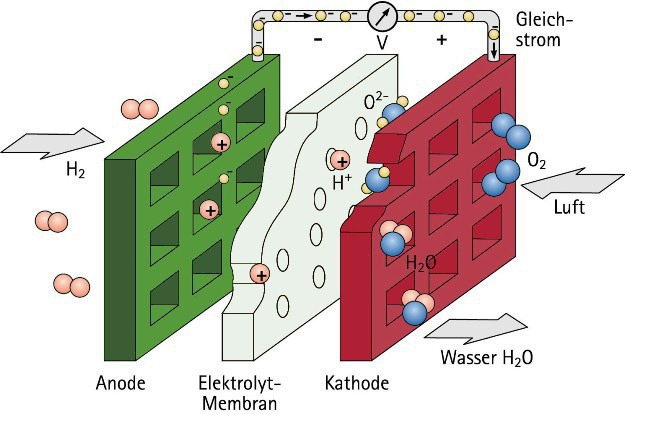
\includegraphics[width=0.6\linewidth]{images/10_Wasserstoffzelle.png}
\end{figure}

Reaktionen der $H_2$-Brennstoffzelle:
\begin{table}[htbp]
	\begin{tabular}{llll}
		Anode (-): & $H_2$ & $\rightarrow$ & $2 H^+ + 2 e^-$ \\
		Kathode (+): & $\frac{1}{2} O_2 + 2 e^-$ & $\rightarrow$ & $O^{2-}$ \\ \hline
		Gesamt: & $H_2 + \frac{1}{2} O_2$ & $\rightarrow$ & $H_2O$
	\end{tabular}
\end{table}

Spannung: \\
$E_{H2/H+} = -0.06V \cdot pH$ \\
$E_{H2O/O2} = 1.23V - 0.06V \cdot pH$ \\
$\Rightarrow \Delta E = 1.23 V$ \\

Aufbau einer polymer elektrolyte fuel cell (PEFC):
\begin{itemize}
	\item Polymermembran als Elektrolyt
	\item Elektroden aus Graphit
	\item Katalysatoren (Pt für Kathode, Pt/Ru für Anode)
	\item Gasdiffusionslage (GDL): poröses Graphitgeflecht für Verteilung der Gase, $e^-$-Leitung und Abtransport des $H_2O$
	\item Bipolarplatten aus Metall oder Graphit für Gaszuführung
\end{itemize}